La transmission sans-fil du code Manchester est assur�e par une combinaison LED-photor�cepteur. La LED est situ�e sur le dessus de la station de recharge et le photor�cepteur est situ� sur le dessus du robot. Ce syst�me de communication sans-fil est limit� � des distances relativement faibles, mais le robot �tant en contact physique avec la station de recharge, cette contrainte ne pose pas de probl�me. Le dessin 3D pr�sent� pr�c�demment servira � planifier la disposition exacte de ces composantes une fois les pi�ces re�ues et le concept test� de mani�re � minimiser les temps de construction et d'assemblage.

\medbreak

La LED est modul� par un microcontr�leur situ� sur la station de recharge. Le mod�le du microcontr�leur reste � d�terminer, mais devra �tre assez simple et peu co�teux puisque sa t�che sera relativement simple. Ce syst�me de communication est illustr� sur le sch�ma \ref{f:led_robot}.

\medbreak

Le document \cite{COM00} explique bri�vement comment r�aliser un tel syst�me et est utilis� comme r�f�rence pour r�aliser notre syst�me.


\begin{figure}[htp]
	\centering
	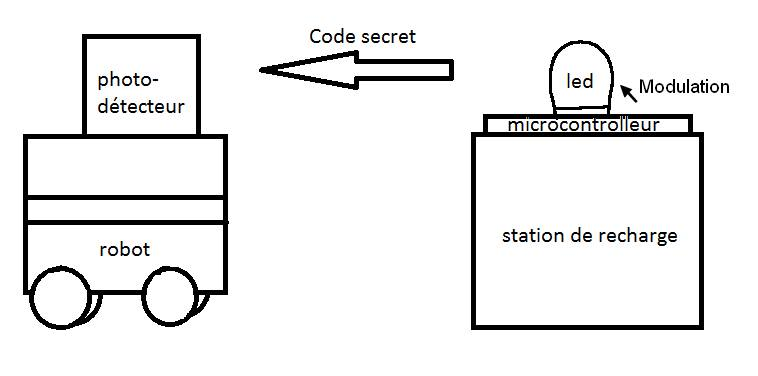
\includegraphics[scale = 0.4]{fig/led_robot.png}
	\caption{Communication sans-fil entre la station de recharge et le robot}
	\label{f:led_robot}
\end{figure}